%% 
%% Copyright 2007-2020 Elsevier Ltd
%% 
%% This file is part of the 'Elsarticle Bundle'.
%% ---------------------------------------------
%% 
%% It may be distributed under the conditions of the LaTeX Project Public
%% License, either version 1.2 of this license or (at your option) any
%% later version.  The latest version of this license is in
%%    http://www.latex-project.org/lppl.txt
%% and version 1.2 or later is part of all distributions of LaTeX
%% version 1999/12/01 or later.
%% 
%% The list of all files belonging to the 'Elsarticle Bundle' is
%% given in the file `manifest.txt'.
%% 
%% Template article for Elsevier's document class `elsarticle'
%% with harvard style bibliographic references

%\documentclass[preprint,12pt,authoryear]{elsarticle}

%% Use the option review to obtain double line spacing
%% \documentclass[authoryear,preprint,review,12pt]{elsarticle}

%% Use the options 1p,twocolumn; 3p; 3p,twocolumn; 5p; or 5p,twocolumn
%% for a journal layout:
%% \documentclass[final,1p,times,authoryear]{elsarticle}
%% \documentclass[final,1p,times,twocolumn,authoryear]{elsarticle}
%% \documentclass[final,3p,times,authoryear]{elsarticle}
%% \documentclass[final,3p,times,twocolumn,authoryear]{elsarticle}
%% \documentclass[final,5p,times,authoryear]{elsarticle}
 \documentclass[final,5p,times,twocolumn,authoryear]{elsarticle}

%% For including figures, graphicx.sty has been loaded in
%% elsarticle.cls. If you prefer to use the old commands
%% please give \usepackage{epsfig}

%% The amssymb package provides various useful mathematical symbols
\usepackage{amssymb}
\usepackage{lipsum}
%% The amsthm package provides extended theorem environments
%% \usepackage{amsthm}

%% The lineno packages adds line numbers. Start line numbering with
%% \begin{linenumbers}, end it with \end{linenumbers}. Or switch it on
%% for the whole article with \linenumbers.
%% \usepackage{lineno}

%% You might want to define your own abbreviated commands for common used terms, e.g.:
\newcommand{\kms}{km\,s$^{-1}$}
\newcommand{\msun}{$M_\odot}
\usepackage{float}

%% \journal{New Astronomy}


\begin{document}

\begin{frontmatter}

%% Title, authors and addresses

%% use the tnoteref command within \title for footnotes;
%% use the tnotetext command for theassociated footnote;
%% use the fnref command within \author or \affiliation for footnotes;
%% use the fntext command for theassociated footnote;
%% use the corref command within \author for corresponding author footnotes;
%% use the cortext command for theassociated footnote;
%% use the ead command for the email address,
%% and the form \ead[url] for the home page:
%% \title{Title\tnoteref{label1}}
%% \tnotetext[label1]{}
%% \author{Name\corref{cor1}\fnref{label2}}
%% \ead{email address}
%% \ead[url]{home page}
%% \fntext[label2]{}
%% \cortext[cor1]{}
%% \affiliation{organization={},
%%            addressline={}, 
%%            city={},
%%            postcode={}, 
%%            state={},
%%            country={}}
%% \fntext[label3]{}

\title{Detecting Gamma-Ray Bursts from Star Explosions}

%% use optional labels to link authors explicitly to addresses:
%% \author[label1,label2]{}
%% \affiliation[label1]{organization={},
%%             addressline={},
%%             city={},
%%             postcode={},
%%             state={},
%%             country={}}
%%
%% \affiliation[label2]{organization={},
%%             addressline={},
%%             city={},
%%             postcode={},
%%             state={},
%%             country={}}

\author[first]{Jaiden Lin}
\affiliation[first]{organization={Institute for Computing in Research},%Department and Organization
            city={Portland},
            state={Oregon},
            country={US}}

\begin{abstract}
%% Text of abstract
Gamma-ray burst that come from space are detected by our satellites in time series, data sets based on time. In order to find the bursts with easier than by eye, an algorithm can be made to detect long and short gamma-ray bursts. Developing four methods, the goal is to find the starting and ending points of the GRB, which will allow it to be isolated from the background noise. The first method finds the slope between adjacent points and classifies slopes greater than 2000 as anomalies; the second method compares the mean of a 5-second interval with the previous interval's mean plus three times the STD of that interval and classifies the interval as anomalies if the mean is greater than the latter; the third method assumes the first fifty seconds of the time series is background noise and subtracts that from the data to find GRBs that are still positive; the fourth method uses a sliding interval that increases in size in order to find the starting point where intervals have the greatest mean. The results of all four were similar, but the fourth method was best because it did not make assumptions and could find both the starting and ending times. Further development of the algorithm would be to apply the fourth method to other time series with different sized and multiple GRBs.
\end{abstract}

%%Graphical abstract
%\begin{graphicalabstract}
%\includegraphics{grabs}
%\end{graphicalabstract}

%%Research highlights
%\begin{highlights}
%\item Research highlight 1
%\item Research highlight 2
%\end{highlights}

\begin{keyword}
%% keywords here, in the form: keyword \sep keyword, up to a maximum of 6 keywords
GRB - Gamma-Ray Burst \sep STD - Standard Deviation

%% PACS codes here, in the form: \PACS code \sep code

%% MSC codes here, in the form: \MSC code \sep code
%% or \MSC[2008] code \sep code (2000 is the default)

\end{keyword}


\end{frontmatter}

%\tableofcontents

%% \linenumbers

%% main text

\section{Introduction}
Ever since the discovery of gamma-ray bursts (GRBs) originating from beyond our planet in 1963, scientists have been intrigued in where these bursts are coming from, what causes such bursts, and what is the science behind these powerful jets. Since then, multiple satellites have been sent into space to monitor the gamma radiation that is directed towards Earth with the data collected in time series, a type of dataset which tracks a sample over time. Collecting data for each individual photon detected in the burst on contact, the time series ensures that it is in terms of time before keeping track of the energy of each photon, and the x and y positions of the photon. The issue is that navigating through  that data is tedious and difficult to search all the bursts by eye. There are some occurrences where the spike just barely exceeds the background noise; this is one of the cases where searching gamma-ray bursts by eye is not optimal. Therefore, as the objective of this study, by programming an automated process that can detect different types of GRBs on its own, it would lessen the time-consuming work of scientists searching through the entire time series. For this to be done, finding the start and end point of a burst is crucial and requires statistical analysis without making assumptions of the background noise, the variability of the burst, and the shape of the burst.

\section{Background information}
To understand the causes and history behind gamma-ray bursts, it is important to have insight of the physics and astronomy behind it.
\subsection{Discovery}
Gamma-rays, more commonly known as gamma radiation and represented by the gamma character of the Greek alphabet, consist of photons with the shortest wavelength, fastest frequency, and highest energy out of any other type from the light spectrum. A well-known source of gamma radiation invented by humans is nuclear weaponry. Nuclear weaponry was a matter of conflict during the Cold War between America and the Soviet Union, and an attempted solution to the weapons race was the "Partial Test Ban Treaty" of 1963. This treaty between the two world superpowers was made to prevent further nuclear weapon testing. Despite the treaty, the United States did not trust the USSR to follow the treaty and thus, sent Vela spy satellites made in the Los Alamos laboratories into space to monitor the Soviet's gamma-rays. However, when they received the data, they were shocked to find massive spikes of gamma-rays that exceeded any nuclear weapon known at that time. It was found that these "bursts" did not come from anywhere on Earth or the Moon, but farther than that. Seeing this anomaly, the Los Alamos laboratories went on a tangent to further investigate these gamma-ray bursts of cosmic origin, publishing their discoveries in 1973. \citep{history}
As many following satellite missions dedicate instrumentation to detecting gamma-rays, there were more and more samples of cosmic bursts. But the catch was that there didn't seem to be a correlation between them. (Figure 1.)
\begin{figure}[H]
	\centering 
	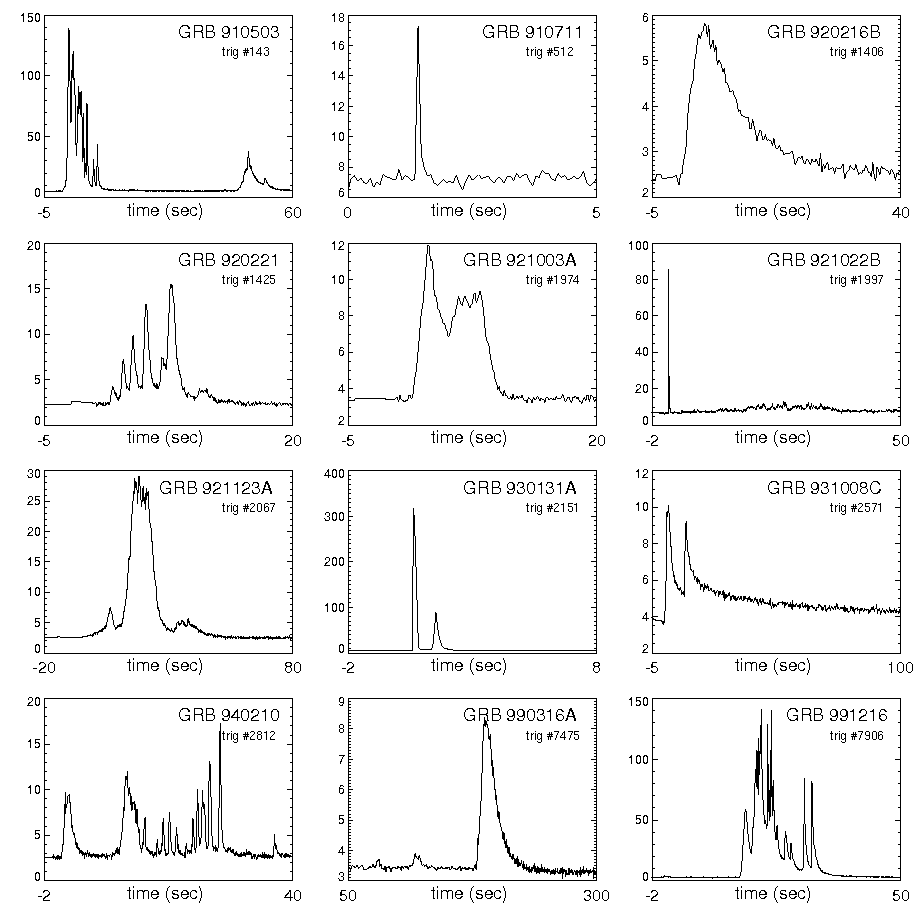
\includegraphics[width=0.4\textwidth]{images/GRB_BATSE_12lightcurves.png}	
	\caption{Various gamma-ray bursts} 
	\label{fig_mom0}%
\end{figure}
It was also found from a sky distribution scatter plot that the bursts we detect can be from beyond our galaxy, not necessarily required for it to be originating from the two-dimensional view we have of our Milky Way. Bursts from far far away show up in the data and can be just as great as bursts in our galaxy.
\subsection{Classification}
So if cosmic gamma-ray bursts can come from anywhere and there's no definite pattern, where do they come from? The likely answer is that stars cause these bursts through an explosive reaction which depends on what type of burst, long or short. Long gamma-ray bursts originate from Type II supernovas, occurring when the mass of a giant star is too much for the core to handle and the star collapses in on itself. All the mass of the star's outer layers crushes the core into either a neutron star or a black hole, depending on its mass where it results in the latter if there is a greater amount of mass prior the supernova.
For short gamma-ray bursts, they come from three types of "mergers": neutron start-neutron star, neutron star-black hole, and black hole-black hole. All three of these mergers result in a black hole as the two celestial objects rotate around each other, getting closer and closer from each other's gravitational pull. On collision, the former two (neutron start-neutron star, neutron star-black hole) combust into a "kilonova" where it spews out all the interior material of the neutron stars. On the other hand, when a binary black hole system collides, they merge together to form a bigger black hole. Although, this variation does not include an astronomical explosion, it still generates the energy necessary for a gamma-ray burst. \citep{mergers}
\subsection{Detection}
Black holes, theorized as regions of space-time with such powerful gravity that light or electromagnetic waves do not have the energy to escape it, are the greatest cause for the gamma-ray bursts that we detect. After the initial event, whether it's long or short, the core—now black hole—will shoot out all the remaining surrounding energy from its poles as the black hole rotates at extreme speeds. These jets that spew out the guts of the once-living star shoots more energy in 10 seconds than the Sun will emit in its entire 10 billion-year lifetime. This also introduces the condition that in order for our satellites to detect gamma-ray bursts, the jet must be pointed in our general direction. Since we are so far away from the source, this makes sense as the burst needs to travel a long ways away, which lessens its energy as it gets farther and farther away.
With vast possibilities in outer space, the condition that a gamma-ray burst has to be directed towards Earth doesn't make it any rarer as the rate is approximately one burst per day. 

\section{Materials}
Satellites often collect data on gamma-ray bursts using time series: data sets that observe a sample based on time. The time series I used came from the Swift satellite's official website. From there, the data was filtered as to isolate the large gamma-ray burst that we will experiment on first. Some components used for programming include a Linux-running laptop and Jupyter notebook as the workspace for writing the algorithm. Libraries used in the code include: NumPy, for high-level mathematical functions; MatPlotLib, a plotting library; Pandas, a data analysis and manipulation tool; AstroPy, for astronomy (specifically, time series) \citep{astropy:2013} \citep{astropy:2018} \citep{astropy:2022}.
\begin{figure}[H]
	\centering 
	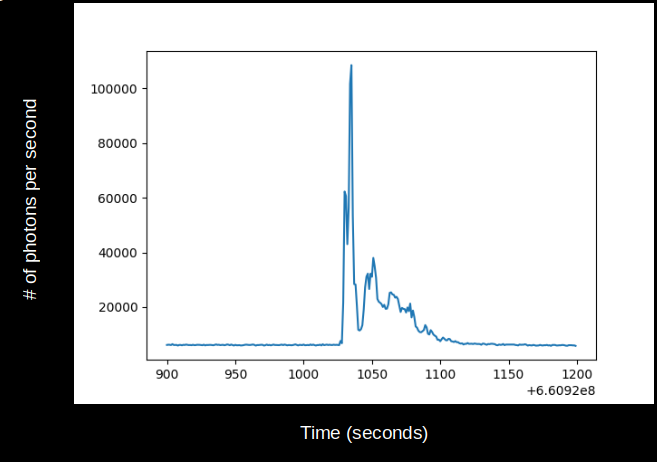
\includegraphics[width=0.4\textwidth]{images/TimeSeries.png}	
	\caption{Time series from the Swift satellite} 
	\label{fig_mom0}%
\end{figure}

\section{Graphs}
First, to experiment with the data set's variables, graphs were made to strengthen the insight of the data and give us a visualization of how a gamma-ray burst can stand out from the background noise.
\subsection{Scatter Plots}
The scatter plots had the x-axis as the x position and y-axis as the y position of each individual photon while the size represented their energy. These plots were produced from MatPlotLib and are accompanied by a slider that changes the time that the plot is at based on seconds. From the plots, it can be seen that at the assumed start time based off seeing the time series histogram (Figure 2), the observed field is much more filled than the initial time (Figure 3). However, it is rather difficult to make any conclusions on the count of photons present when the plotted dots are overlapping with each other. Therefore, a different type of graph would be more efficient.
\begin{figure}[H]
	\centering 
	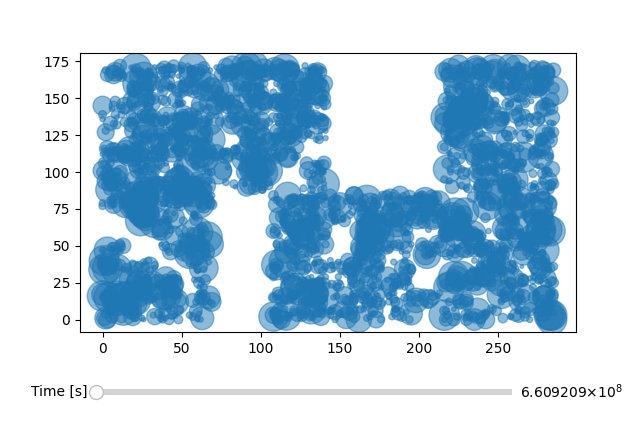
\includegraphics[width=0.4\textwidth]{images/ScatterPlot.png}	
	\caption{Initial scatter plot} 
	\label{fig_mom0}%
\end{figure}
\begin{figure}[H]
	\centering 
	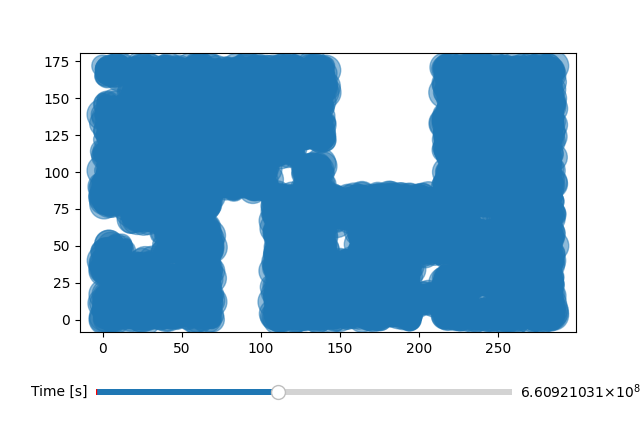
\includegraphics[width=0.4\textwidth]{images/ScatterPlot2.png}	
	\caption{Scatter plot at estimated start time} 
	\label{fig_mom0}%
\end{figure}
\subsection{2D Histograms}
Modeling the time series now in a two-dimensional histogram, each bin would be colored based on how many photons are in that spatial distribution. Similar to the scatter plots, the histogram would be accompanied by a time slider so that the user can view the field at different time periods. Based on the distinct difference between the histogram at the initial time (Figure 5) and the histogram at the assumed start time of the burst (Figure 6), histograms were found to be much more clear than the adjustable scatter plots. This is because each bin represents a number of photons, making it easier to visualize where photons are concentrated. The only downside to these 2D histograms is that they do not exhibit the variable for each photon's energy.
\begin{figure}[H]
	\centering 
	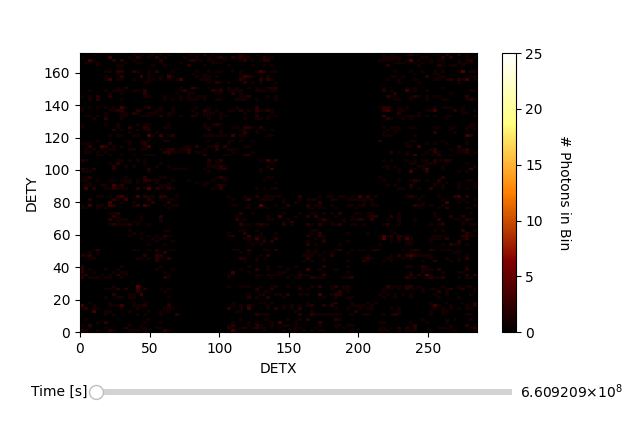
\includegraphics[width=0.4\textwidth]{images/2DHistogram.png}	
	\caption{Histogram at initial time} 
	\label{fig_mom0}%
\end{figure}
\begin{figure}[H]
	\centering 
	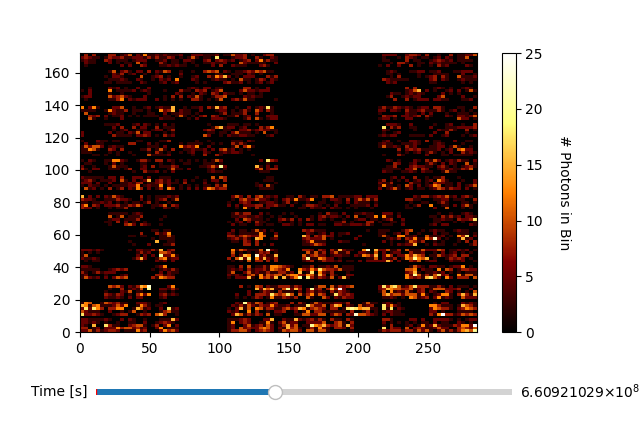
\includegraphics[width=0.4\textwidth]{images/2DHistogram2.png}	
	\caption{Histogram at estimated start time} 
	\label{fig_mom0}%
\end{figure}

\section{Methods}
Moving on to the focus of the study, the idea to code an algorithm that can differentiate a gamma-ray burst from background noise is to find the start time and end time of the GRB. The start time is a distinct and easily-detectable spike in the data, but the data trails off as the GRB comes to an end, making the latter much more difficult to find through an automated procedure. Through experimentation and statistical analysis, four methods were tested total.
\subsection{Finding Slopes}
The first method is to find the slope between two points on the data. For each point in the time series, this method finds the difference of the number of photons between the next second and the current second. If the difference is found to be greater than 2000, then that point would be assumed as an anomaly and possibly part of a gamma-ray burst. From there, the earliest and latest anomalies was taken and the data was filtered to only output data in that range (Figure 7).
\begin{figure}[H]
	\centering 
	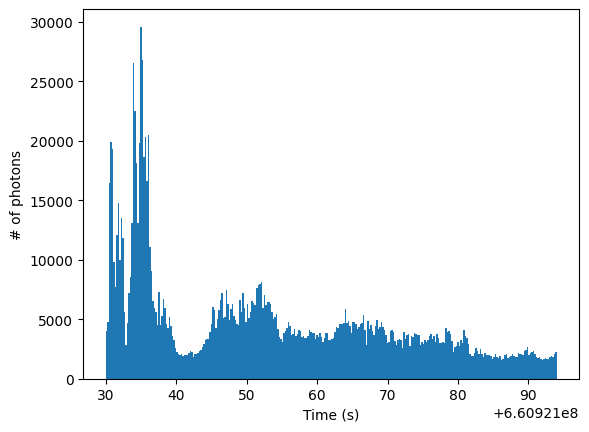
\includegraphics[width=0.4\textwidth]{images/FindingSlopes.png}	
	\caption{Resulting filtered data of Method 1: Finding Slopes} 
	\label{fig_mom0}%
\end{figure}
\subsection{Standard Deviation}
This is not one of the four methods, but is another step that will lead to more. Graphed with the original time series, the mean of each 5-second interval by itself and the mean addition to (or subtracted by) three times the standard deviation of each 5-second interval are graphed as well (Figure 8). These calculations contribute to the statistical analysis of the time series that will be used in the other three methods.
\begin{figure}[H]
	\centering 
	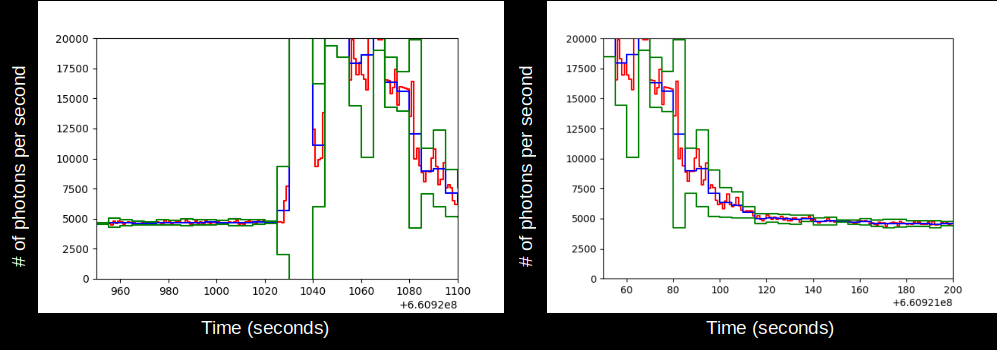
\includegraphics[width=0.4\textwidth]{images/STDs.png}	
	\caption{Red is the data; blue is the mean of the 5-second intervals; green is the mean +/- three times the standard deviation} 
	\label{fig_mom0}%
\end{figure}
\subsection{Comparing Means to STDs}
This method is similar to the first as it compares the data from one second to an adjacent second, but in contrast, the second method compares the mean of the current 5-second interval to the previous 5-second interval's mean + three times its standard deviation. The earliest and latest anomalies are also assumed to be the starting and ending points of the burst and the data is filtered (Figure 9).
\begin{figure}[H]
	\centering 
	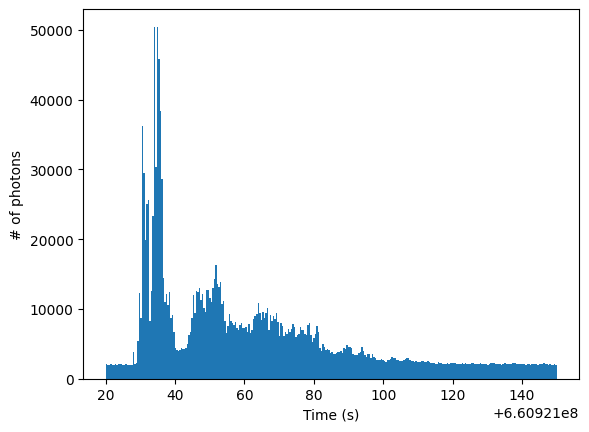
\includegraphics[width=0.4\textwidth]{images/CompareMeanToSTD.png}	
	\caption{Resulting filtered data of Method 2: Comparing Means to STDs} 
	\label{fig_mom0}%
\end{figure}
\subsection{Assuming the Background}
The third method uses the mean of the first fifty seconds of the time series plus three times the standard deviation of the fifty seconds. The sum is declared as the background noise and the value is subtracted from the entirety of the time series. This would result in the removal of the background noise, leaving only gamma-ray bursts to be above zero. This makes it much easier to detect the entirety of gamma-ray bursts that transcend the background noise.
\begin{figure}[H]
	\centering 
	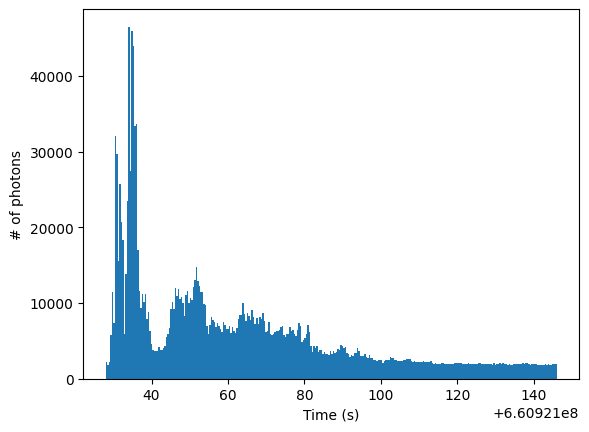
\includegraphics[width=0.4\textwidth]{images/FiftySecBG.png}	
	\caption{Resulting filtered data of Method 3: Assuming the Background} 
	\label{fig_mom0}%
\end{figure}
\subsection{Sliding Frame}
The most complex method of the four, it utilizes loop functions within loop functions. Starting with an interval of a duration of one second, the interval with the maximum mean of all the 1-second intervals across the time series is recorded in a Pandas dataframe. The duration of the interval is then increased by one each time it goes through the data. As a result, the dataframe would contain intervals of duration from zero to the duration of the entire time series, with one for each of x duration as the mean is maximized. A histogram is then created from the dataframe to find the time period where the most intervals of maximum means starts, essentially finding the starting point for the burst.
\begin{figure}[H]
	\centering 
	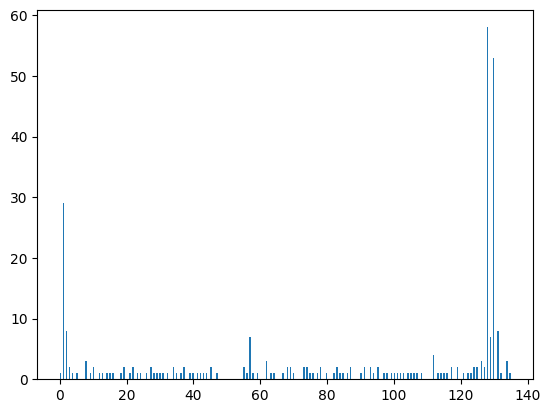
\includegraphics[width=0.4\textwidth]{images/SlidingFrameHist.png}	
	\caption{Histogram of the starting point of all intervals that have the maximum mean out of the intervals with the same duration} 
	\label{fig_mom0}%
\end{figure}
Then, by going through all the maximum mean intervals that start at the declared "starting point of the burst", the interval with the maximum duration is chosen as the interval where the gamma-ray burst resides in.
\begin{figure}[H]
	\centering 
	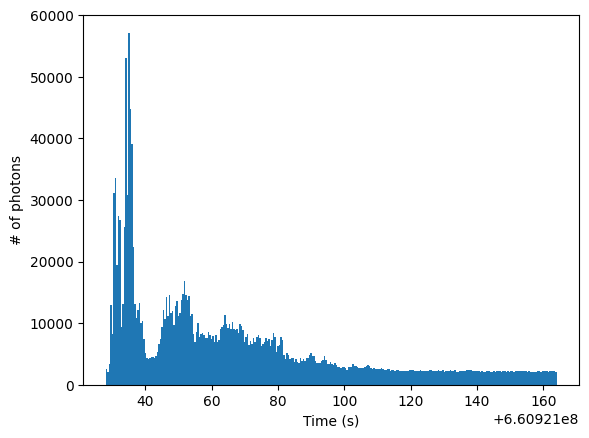
\includegraphics[width=0.4\textwidth]{images/SlidingFrame.png}	
	\caption{Resulting filtered data of Method 4: Sliding Frame} 
	\label{fig_mom0}%
\end{figure}

\section{Discussion}
From the results of all four methods, it can be said that they all produce satisfying results. However, the procedures that find the starting and ending points of the gamma-ray burst is different and may not work as well if applied to other time series. The issue of the first method, Finding Slopes, is that it doesn't count sections in the burst as anomalies if the change between adjacent data is not significant enough. Therefore, this is not the optimal method. The second method, Comparing Means to STDs, also exhibits the same problem as the first, incapable of detecting some sections in the burst as anomalies because the change is not significant enough. The third method, Assuming the Background, is the best one yet, but the only complication is that the algorithm assumes that the first fifty seconds of the time series is entirely background noise. If a gamma-ray burst was to occur within that time frame, this method would be defective. And out of the four methods, the fourth one, Sliding Frame, seemed to be the best as it doesn't make any assumptions and it finds the starting and ending points efficiently. The only difficulty is that this method is not applicable to time series where multiple gamma-ray bursts are present, which, on the other hand, is an advantage that the third method has over the fourth.

\section{Conclusion}
Experimenting through the various methods, the results may be sufficient, but the proficiency of the processes can vary. The fourth method seems to be the best of the four, but it has its disadvantages as well. Therefore, in order to improve this study's algorithm for detecting gamma-ray bursts, the next steps are to test these methods on other time series. Using them on different shapes of gamma-ray bursts  or even multiple GRBs would build more insight in how the methods work well or don't work well with variations of data. So, improvements to the algorithm can be made if further research is possible to produce a final algorithm that can effectively detect the time period of gamma-ray bursts. This study is significant in that it attempts to create an easier process to detect gamma-ray bursts, long and short, Furthermore, helping the study of GRBs may inform us more of stellar evolution, the way stars live, work, and die. It may also teach scientists more of unique cases such as mergers, black holes, and star systems both singular and binary. By analyzing time series with algorithms, the project displays experimentation with our current cosmological technology that may allow us to further develop our instruments so that we can discover even more about the mysteries beyond our solar system.


\section*{Acknowledgements}
Thank you to my mentor, Aaron Tohuvavohu, for your guidance throughout this project and thank you to the Institute for Computing in Research to making this possible.


\bibliographystyle{elsarticle-harv} 
\bibliography{example}


\end{document}

\endinput
%%
%% End of file `elsarticle-template-harv.tex'.
